\documentclass[10pt, xcolor=table]{beamer}

\setbeamertemplate{note page}[default]
%\setbeameroption{hide notes}
\setbeameroption{show notes}
\setbeamerfont{footnote}{size=\tiny}

\usetheme[progressbar=frametitle]{metropolis}
\usepackage{appendixnumberbeamer}

\usepackage{booktabs}
\usepackage[scale=2]{ccicons}

\usepackage{pgfplots}
\usepgfplotslibrary{dateplot}
\usepackage{multicol}
\setlength{\columnsep}{1.5cm}
\usepackage{multirow}

\usepackage{hyperref}
%\usepackage{animate}
\usepackage{lmodern}
\usepackage[T1]{fontenc}
\usepackage{mathtools}
\usepackage{graphicx}
\usepackage[font=scriptsize]{caption}
\usepackage{tikz}
\usepackage{stackengine}
\usepackage{array}
\usetikzlibrary{positioning}
\usepackage{tabularx}
\usepackage{tabulary}
%\hypersetup{
%    colorlinks=true,
%    linktoc=none,
%    linkcolor=blue,
%    urlcolor=blue
%}

\usepackage[math]{cellspace}
\cellspacetoplimit 2pt
\cellspacebottomlimit 2pt


%\definecolor{set1}{RGB}{228, 26, 28}
%\definecolor{set2}{RGB}{77, 175, 74}
%\definecolor{set3}{RGB}{255, 127, 0}
%\definecolor{set4}{RGB}{166, 86, 40}
%\definecolor{set5}{RGB}{153, 153, 153}

\usepackage{xspace}
\newcommand{\themename}{\textbf{\textsc{metropolis}}\xspace}

\newcommand\Fontvi{\fontsize{8}{9}\selectfont}
\newcommand\Fontvr{\fontsize{6}{7}\selectfont}

\setbeamerfont{parent A}{size=\small}

\DeclarePairedDelimiter\abs{\lvert}{\rvert}%
\DeclarePairedDelimiter\norm{\lVert}{\rVert}%
\makeatletter
\let\oldabs\abs
\def\abs{\@ifstar{\oldabs}{\oldabs*}}
\let\oldnorm\norm
\def\norm{\@ifstar{\oldnorm}{\oldnorm*}}
\makeatother
\newcommand*{\Value}{\frac{1}{2}x^2}%

\newcommand{\floatfootnote}[1]{\ifx\[$\else\footnote{#1}\fi}
\newcommand{\floatfootnotes}[1]{\ifx\[$\else\footnote{#1}\fi}



\title{Digital Transformation of Healthcare}
\subtitle{Economic Valuation}
% \date{\today}
\date{}
\author{Michoel Snow, M.D. Ph.D., Glen Ferguson, Ph.D.}
\institute{Center for Health Data Innovations}
% \titlegraphic{\hfill\includegraphics[height=1.5cm]{logo.pdf}}

\begin{document}

\maketitle


\begin{frame}{Economic Valuation}
	After this lecture students will be able to 
	\begin{itemize}
		\item Define the costs associated with an intervention
		\item Differentiate between direct and indirect costs 
		\item Locate estimates for direct and indirect costs
		\item Discuss Markov Chain Monte Carlo for modeling costs
	\end{itemize}
\end{frame}


\begin{frame}{Bioinformatics Pipeline}
	\begin{center}
		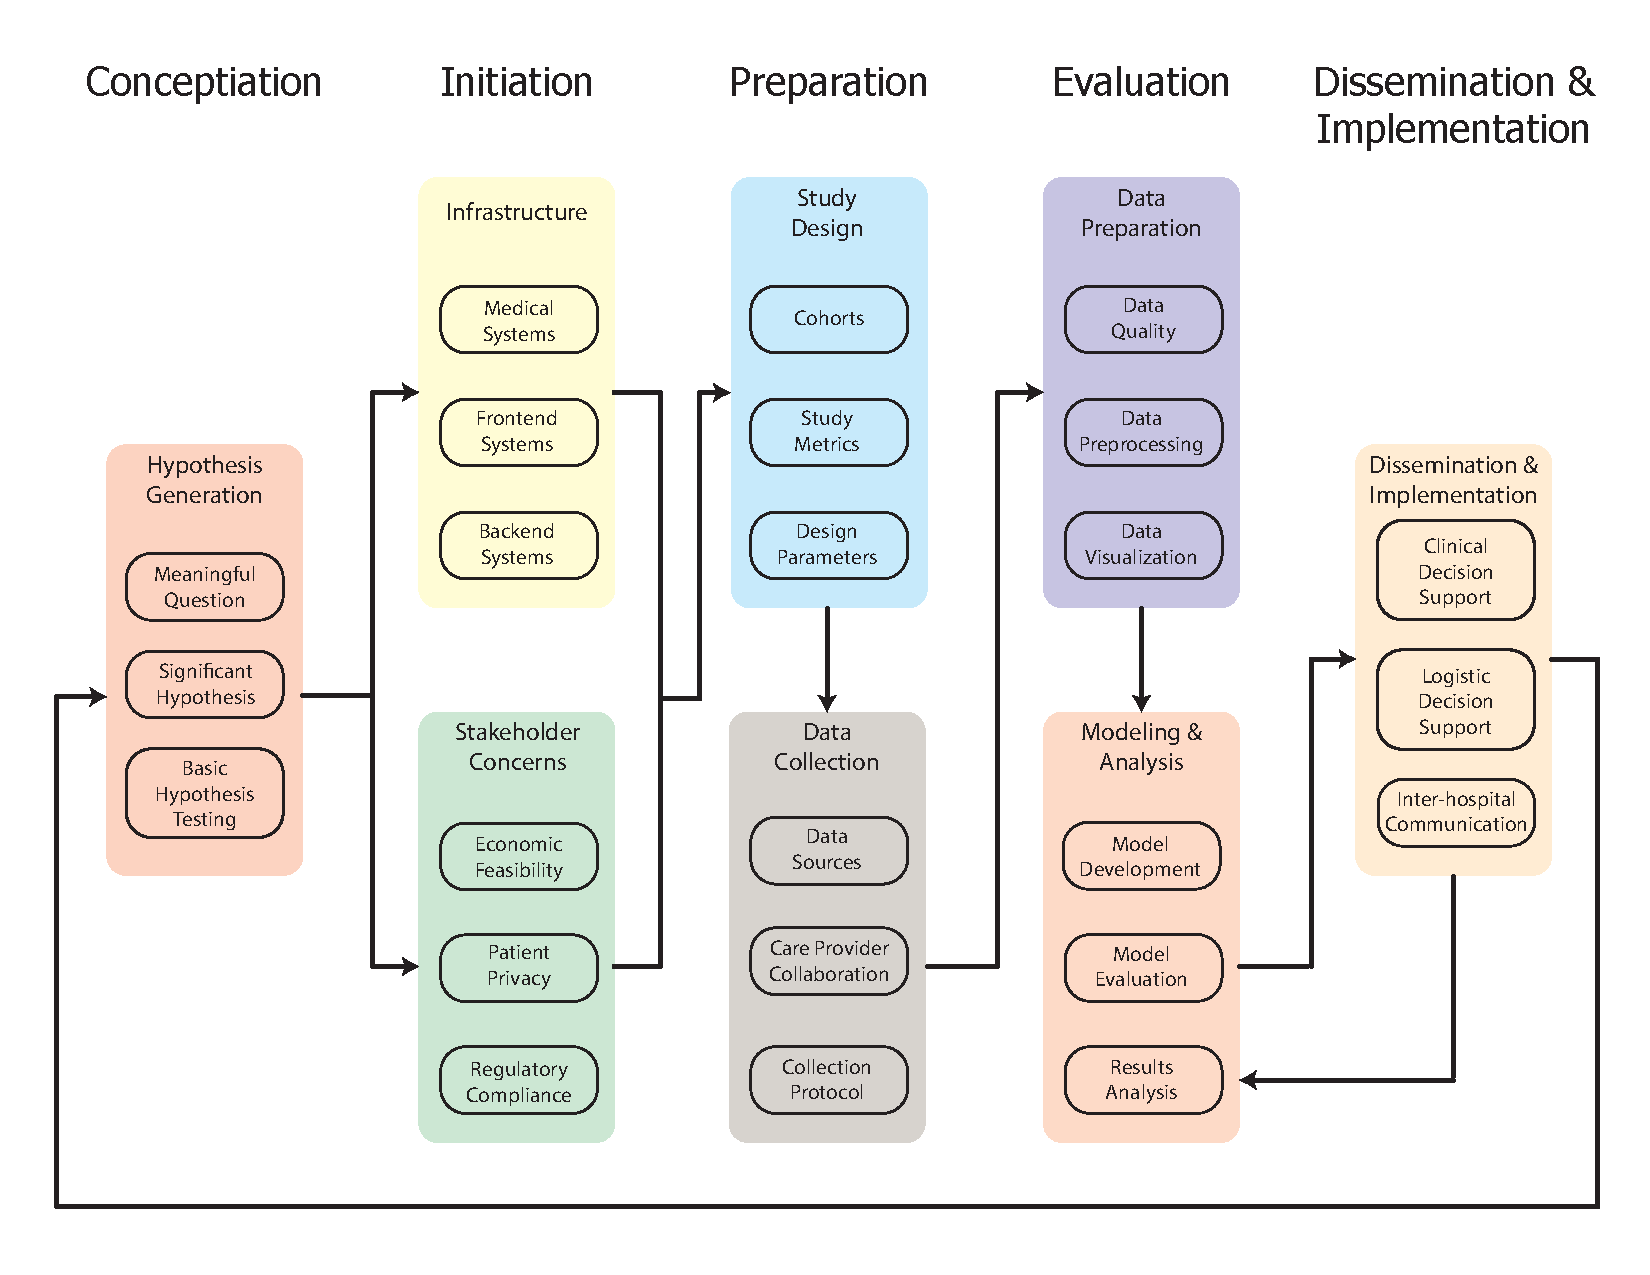
\includegraphics[width=0.9\textwidth]{images/informatics_pipeline.pdf}	
	\end{center}
\end{frame}


\begin{frame}{Economic Valuation}
	\begin{center}
		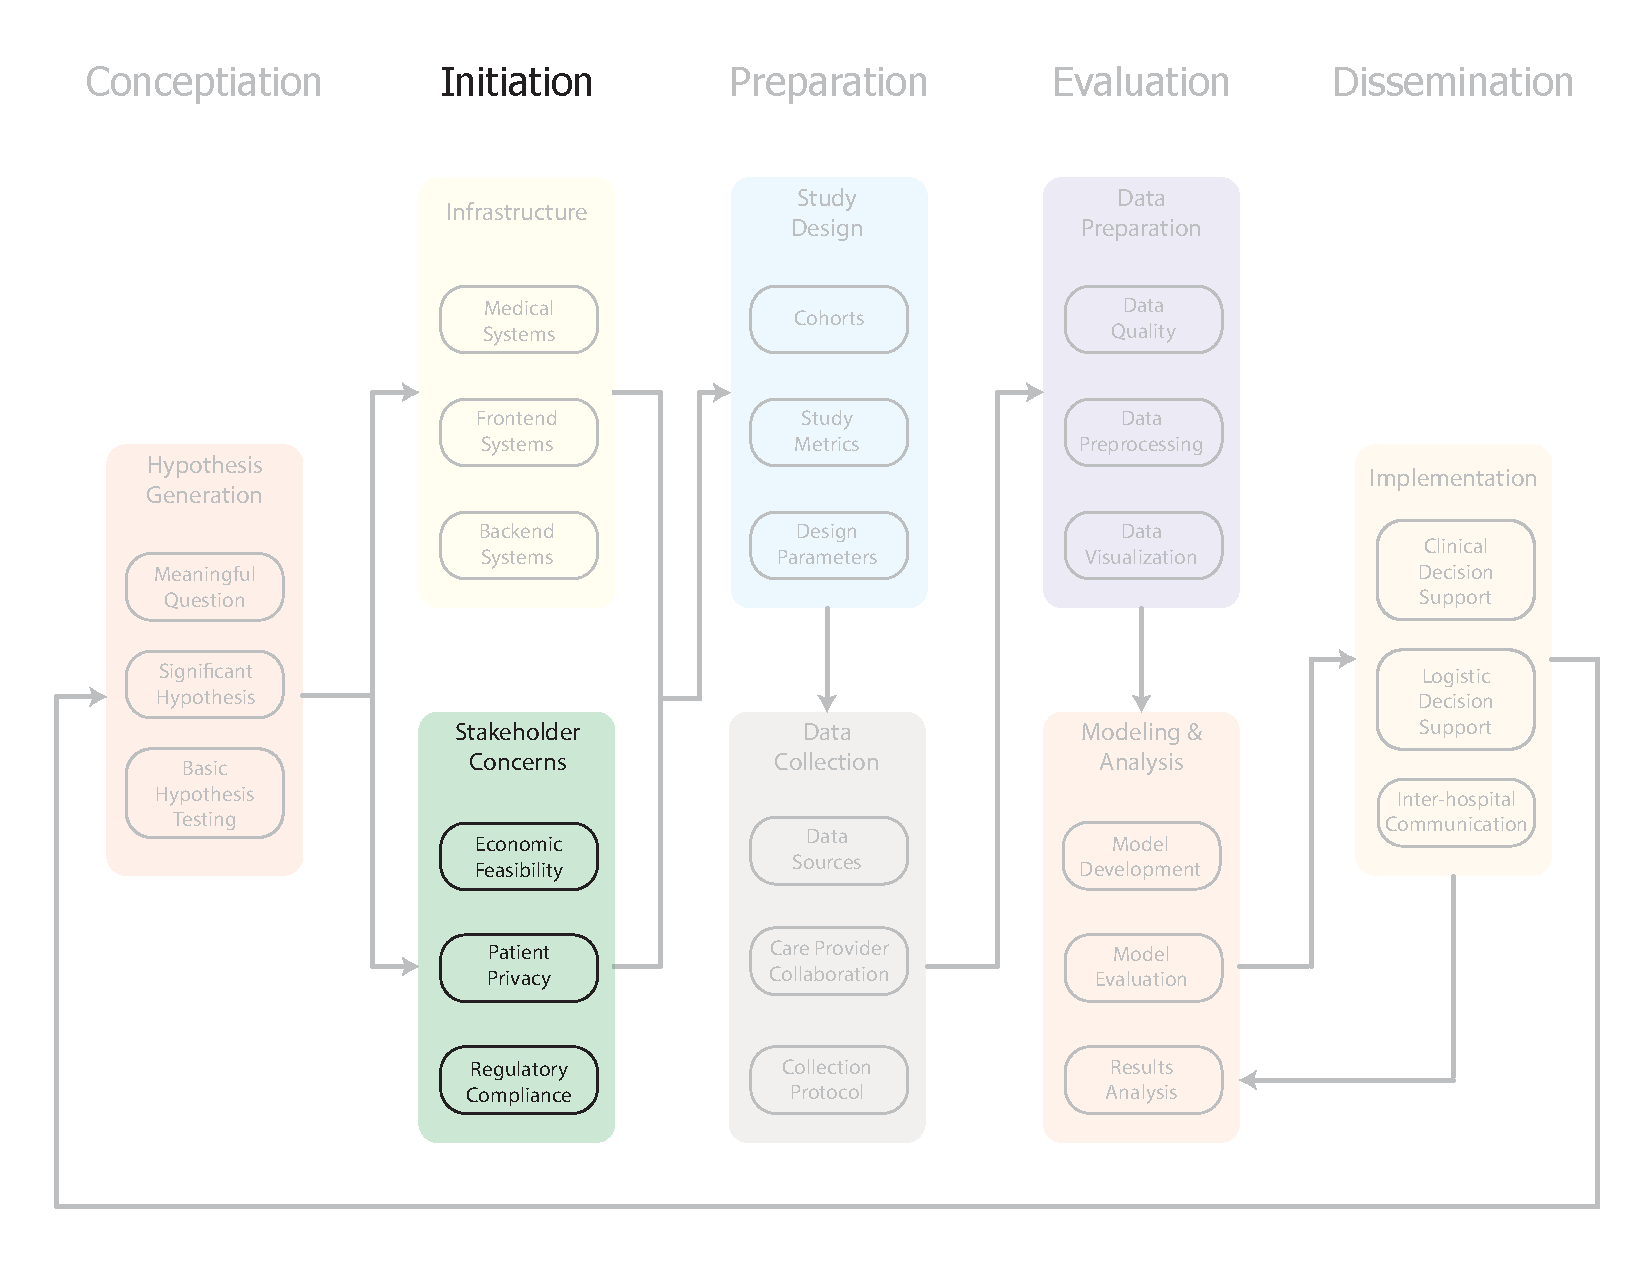
\includegraphics[width=0.9\textwidth]{images/informatics_pipeline_econ_value.pdf}	
	\end{center}
\end{frame}


\begin{frame}{Scenario}
	\begin{itemize}
		\item You have some new radical ideas for the diagnosis and management of stroke.
		\item Before you begin you are tasked with providing a cost-benefit analysis for the department.
		\item How can you quantify the costs and benefits of your new protocol as compared to the current standard of care?
		\item How can you use the costs to determine the benefit of any new intervention.
%		\begin{itemize}
%			\item What are the steps to transform raw data into a usable format
%		\end{itemize}
	\end{itemize}
%	\begin{center}
%		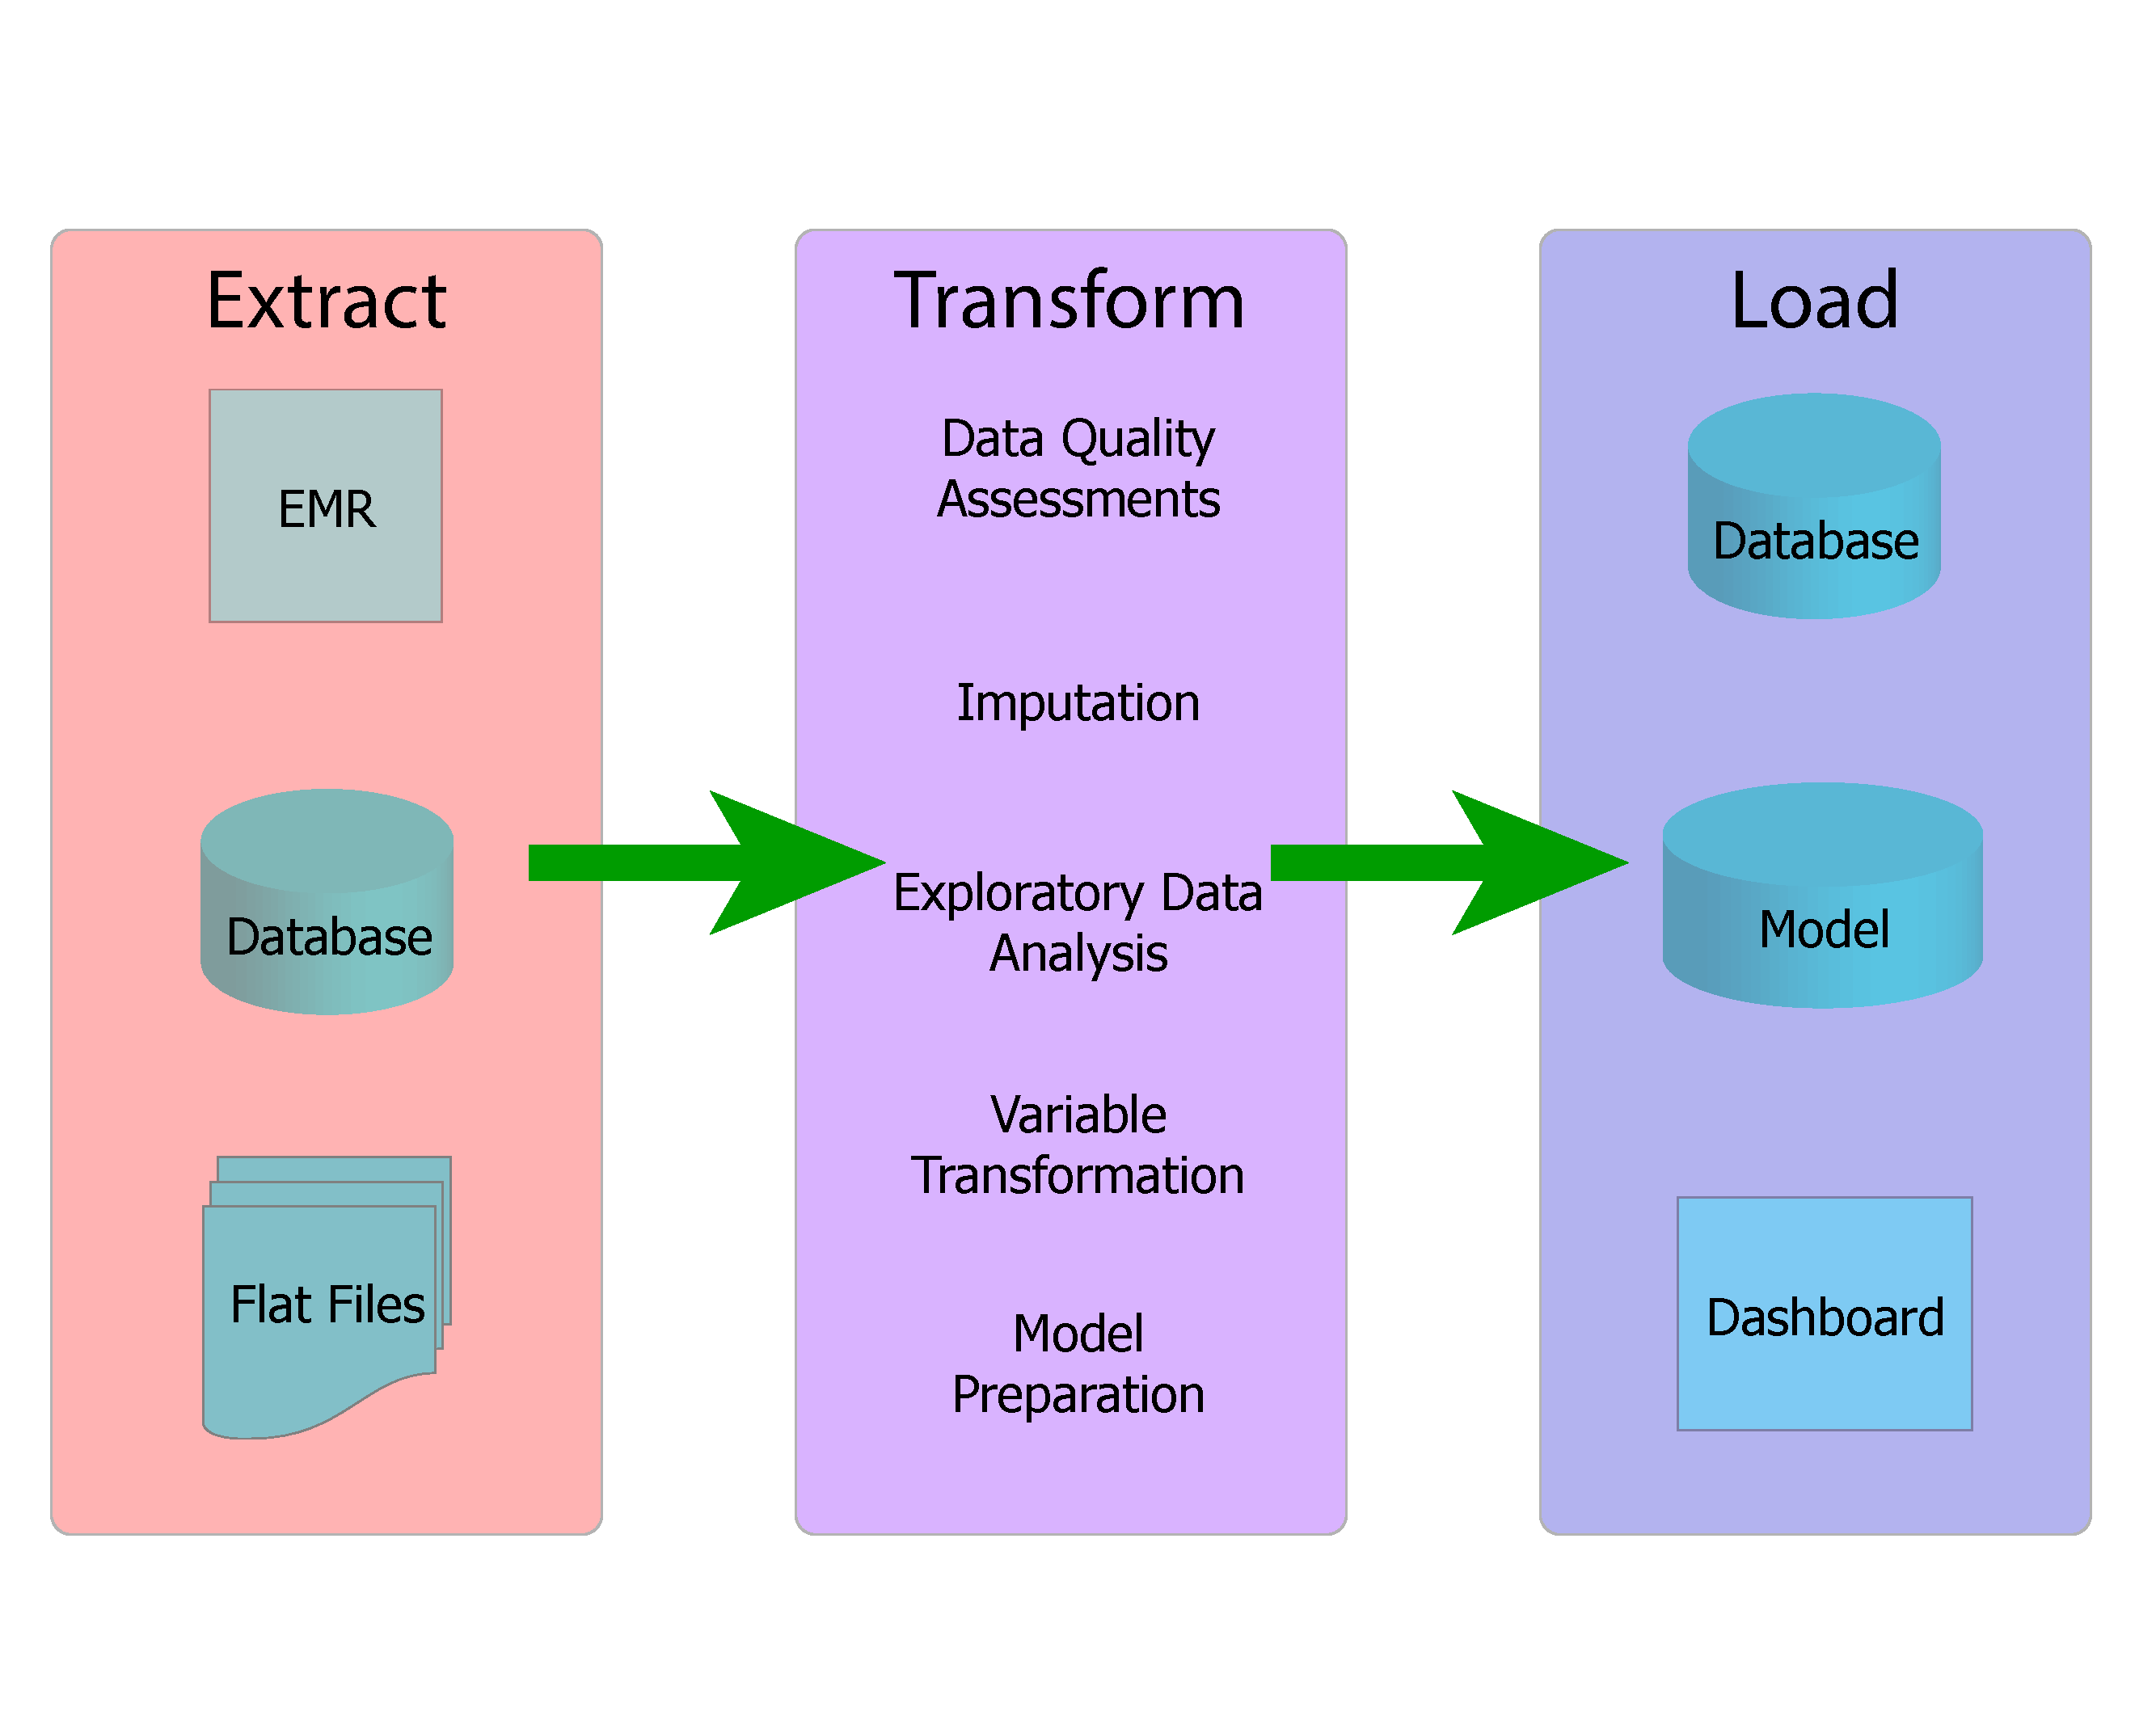
\includegraphics[width=0.5\textwidth]{images/etl.pdf}	
%	\end{center}
\end{frame}

\note{
	\scriptsize
	\begin{itemize}
		\item Costs
		\begin{itemize}
			\scriptsize
			\item Cost parameters - (cost of any intervention D+, cost of any intervention D-, cost of missed)
			\item Direct costs - Hospital (Medication, testing, Tx, length of stay, doctors, nurses other support staff, other services, e.g., food, transport, ambulance services, initial hospitalization, inpatient and outpatient rehabilitation services including durable medical equipment, nursing home costs, and outpatient neurology clinic visits)
			\item Indirect costs - Loss or work, Quality of life (QALY)
			\item Other - Litigation
		\end{itemize}
		\item  (intervention1 - intervention2)/(Increase in QOL1 - Increase in QOL2)
	\end{itemize}

}


\begin{frame}{Projected costs of ischemic stroke in the United States \footnote{D. L. Brown, B. Boden-Albala, K. M. Langa, L. D. Lisabeth, M. Fair, M. A. Smith, R. L. Sacco, L. B. Morgenstern
Neurology Oct 2006, 67 (8) 1390-1395; DOI: 10.1212/01.wnl.0000237024.16438.20}}
	\begin{itemize}
		\small
		\item \textbf{Objective} - To estimate the future economic burden of stroke in non-Hispanic whites, Hispanics, and African Americans in the United States from 2005 to 2050.
		\item \textbf{Methods} -  We used U.S. Census estimates of the race–ethnic group populations age 45 years and older. We obtained stroke epidemiology and service utilization data from the Northern Manhattan Stroke Study and the Brain Attack Surveillance in Corpus Christi project and other published data. We estimated costs directly from Medicare reimbursement or from studies that used Medicare reimbursement. Direct and indirect costs considered included ambulance services, initial hospitalization, rehabilitation, nursing home costs, outpatient clinic visits, drugs, informal caregiving, and potential lost earnings.
	\end{itemize}
	
\end{frame}

\begin{frame}{Estimate of Direct Costs}
	\scriptsize
	\begin{itemize}
		\item \textbf{Ambulance} - The proportions of ischemic stroke patients in each race–ethnic group arriving by ambulance were estimated from BASIC. Average allowable costs reimbursed by Medicare were used to estimate ambulance costs\footnote{\label{note1}http://www.cms.hhs.gov}.
		\item \textbf{Inpatient} - All patients were assumed to be hospitalized for any incident ischemic stroke. Costs were estimated from the literature\footnote{Samsa GP, Bian J, Lipscomb J, Matchar DB. Stroke 1999;30:338–349.}.
		\item \textbf{Inpatient Rehab} - For each race–ethnic group, the proportion of stroke patients admitted for inpatient rehabilitation was calculated from the weighted average of NOMASS and BASIC stroke patients. Costs were based on maximum allowable Medicare reimbursement for rehabilitation\footnotemark[2].
		\item \textbf{Drugs} - Costs of antiplatelets, anticoagulants, antihypertensive, and lipid-lowering agents were considered. The proportions of stroke patients of each race–ethnic group discharged on each medication was obtained from BASIC. The current price of a statin was reduced by two-thirds in anticipation of generic availability in the near future. Drug costs were obtained from the Red Book\footnote{Red Book. Montvale, NJ: Thomson PDR, 2004.}.
		\item \textbf{Direct nonmedical costs: Informal caregiving} - The proportion of stroke patients needing informal caregiving and the hours per day required were estimated from the literature\footnote{Hickenbottom SL, Fendrick AM, Kutcher JS, et al. Neurology 2002;58:1754–1759}. The hourly salary of a home health aide was used to represent the informal caregiving costs\footnote{Gold MR, Siegel JE, Russell LB, Weinstein MC. New York: Oxford University Press, 1996.}.
	\end{itemize}
\end{frame}

\begin{frame}{Estimate of Other Costs}
	\begin{itemize}
		\item Indirect Costs
		\begin{itemize}
			\scriptsize
			\item Indirect medical costs included potential lost earnings.  
			\item Lost earnings were only considered for those younger than 65, as those 65 and older were assumed to be retired. An estimate of the proportion of those in the labor force was calculated based on the race–ethnic-specific employment rate\footnote{http://www.cms.hhs.gov}. 
			\item The proportion assumed to return to work following stroke (53\%) was obtained from the literature\footnote{Wozniak MA, Kittner SJ, Price TR, et al. Stroke 1999;30:2568–2573}.
			\item Individuals were assumed to earn the median salary for each race–ethnic group\footnote{ftp://ftp.bls.gov/pub/special.requests/lf/aat37.txt}.
		\end{itemize}
		\item Costs Not Considered
		\begin{itemize}
			\scriptsize
			\item Loss of leisure activities or other activities not related to compensated employment were not included. 
			\item The effects of lost productivity in the work force incurred by others ("friction costs") were also not taken into account in the model.
			\item  Stroke in those less than 45 was also excluded, as estimates of ethnic-specific stroke incidence and prevalence in this age group have not been well studied.
		\end{itemize}
	\end{itemize}
\end{frame}

\begin{frame}{Estimated Costs}
	\begin{center}
		\scriptsize
		\begin{tabular}{lr}
			\toprule
    	\textbf{Service} &  \textbf{Cost per stroke} \\
			\midrule
    	Ambulance &  \$164 \\
    	Hospitalization/emergency dept. & \$12,423 \\
			Rehabilitation inpatient & \$25,968 \\
			Neurologist & \$83 \\
			All therapies, assistive devices, and home health & \$3,218 \\               
			\midrule
			& \textbf{Cost per year} \\
			\midrule
			Aspirin/sustained-release dipyridamole & \$1,543 \\
			Aspirin & \$8 \\
			Clopidogrel & \$1,518 \\
			Warfarin & \$303 \\
			ACE inhibitor & \$384 \\
			Statin & \$437 \\
			PCP & \$53 \\
			Informal care & \$4,038 \\
			Earnings lost & \$22,880 \\
			Nursing home care & \$33,636 \\
			\bottomrule
		\end{tabular}
	\end{center}
\end{frame}

\begin{frame}{Markov Chain Monte Carlo}
	\begin{itemize}
		\item You were able to determine the cost of every single path a patient in the system can take using your new protocol. However, now you have to determine the probability of each patient to follow a specific path
		\item How can you determine what percentage of patients will end up at each of your different end states?
	\end{itemize}
\end{frame}

\note{
	\scriptsize
	\begin{itemize}
		\item Starting from a healthy patient what are the different initial states for your patients - (HTN, diabetes, previous stroke, ...)
		\item What are the different end states for your protocol - (death, persistent vegetative state, Healthy ...)
		\item what are the intermediate stages between the initial and final stage
		\item what are the probabilities of going to each state
	\end{itemize}
}


\end{document}